
Dado que el objetivo del trabajo es mejorar la asignaci\'on de momento para muones high-$p_{T}$, especialmente para los casos con showering, el primer aspecto que se ha de tener en cuenta es recopilar toda la informaci\'on posible del mu\'on (incluyendo los hits que provienen de las cascadas), en contraposici\'on a la estrategia de los distintos refits descritos en la Secci\'on~\ref{sec:current_assignment}, que tratan de encontrar aquellas c\'amaras donde es probable que haya tenido lugar una cascada para despu\'es eliminar la informaci\'on de dichas c\'amaras a la hora de hacer la reconstrucci\'on de la traza del mu\'on.

De esta manera, el procedimiento que se va a seguir para recoger toda la informaci\'on posible es extrapolar la traza del mu\'on medida en el tracker a las c\'amaras de muones, para despu\'es recoger todo el conjunto de hits que se encuentren en torno al punto extrapolaci\'on recogiendo as\'i todas las señales que produzca la posible cascada. \\

En la presente secci\'on se detallar\'an las herramientas y metodolog\'ia utilizadas para el tratamiento de los datos.


\subsection{Herramientas utilizadas para el an\'alisis}\label{sec:tools}

links a Repositorios, CMSSW, root, pandas... etc


\subsection{Selecci\'on de muones y segmentos}\label{sec:selection}


Definir segmentos

FILL ME


\subsection{Muestra de simulaci\'on utilizada}\label{sec:sample}

Se han generado 100000 eventos de $Z'$ con $m_{Z'}$ = 5000 GeV fruto de la colisiones prot\'on-prot\'on a una energ\'ia de centro de masas de 13 TeV (condiciones del acelerador LHC) mediante simulaci\'on de Monte-Carlo utilizando el programa MadGraph5~\cite{Alwall:2014hca}. Se impone que las part\'iculas $Z'$ generadas se desintegren a un par de muones $\mu^{+}\mu^{-}$ y se simula el paso de los muones por el detector CMS con el paquete Geant4~\cite{Agostinelli:2002hh}. De esta manera se tiene una muestra con estad\'istica razonable de muones high-$p_{T}$ con $p_{T}$ generado conocido que se usar\'a para el entrenamiento de la DNN. \\

En la Figura~\ref{fig:data_pt} se muestran las distribuciones del $p_{T}$ generado y el $p_{T}$ proporcionado por el algoritmo TuneP de todos los muones de la muestra que pasan la selecci\'on detallada en la Secci\'on~\ref{sec:selection}.

\begin{figure}[h]
\centering
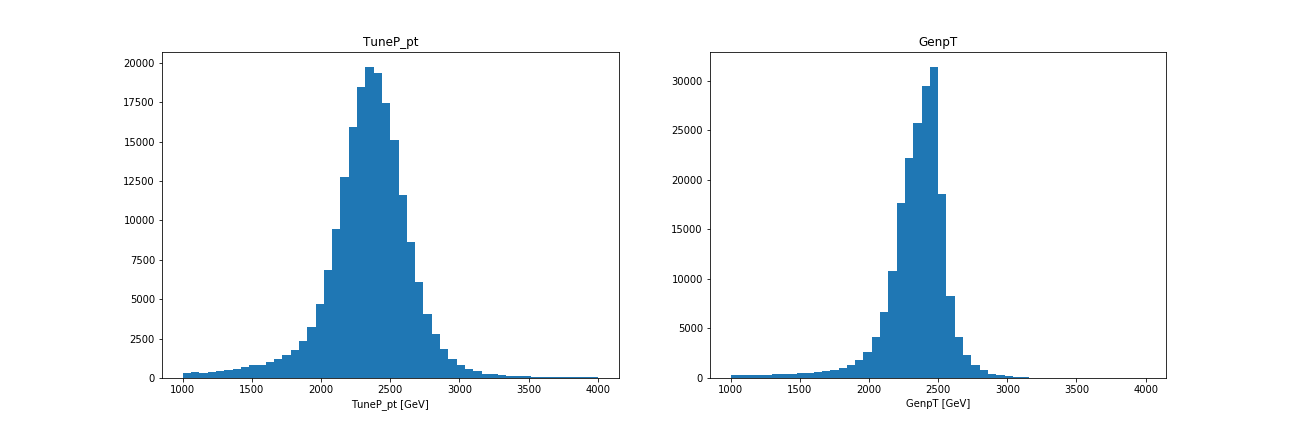
\includegraphics[width=1.0\textwidth]{figures/data_pt.png}
\caption{Distribuciones del momento transverso de los muones de la muestra de simulaci\'on utilizada. Izquierda: $p_{T}$ generado. Derecha: $p_{T}$ proporcionado por el algoritmo TuneP.}
\label{fig:data_pt}        
\end{figure}

\subsection{Distribuciones de control}\label{sec:plots}

FILLME
